\documentclass[11pt]{report}
\usepackage{nopageno} % Disable bottom page #
\usepackage[utf8]{inputenc}
\usepackage{multicol}
\usepackage{titlesec} % title format
\usepackage[top=.5in, left=1in, bottom=1in, right=1in]{geometry}


% Graphics library for displaying pictures
\usepackage{graphicx}
\graphicspath{ {images/} }


% Fix itemize spacing
\newenvironment{myitemize}
{ \begin{itemize}
    \setlength{\itemsep}{0pt}
    \setlength{\parskip}{0pt}
    \setlength{\parsep}{0pt}     }
{ \end{itemize}                  } 

%set font style
\renewcommand\familydefault{\sfdefault}

% Set line spacing
\renewcommand{\baselinestretch}{1}

% Set indent size
\setlength\parindent{0pt}

% Column spacing
\setlength\columnsep{4pt}

% Title formatting
\titleformat{\chapter}{\Huge\bf}{\thechapter}{20px}{\Huge\bf}


\begin{document}
% Begining of title page

{\Huge \textbf{Software Design Document:}}
\vspace{5mm}
\begin{flushright}

    {\huge for}
    \vspace{20mm}

    \textbf{\Huge Vaultron}
    \vspace{20mm}

    {\huge Version $<0.0.1>$}
    \vspace{20mm}

    {\huge Prepared by}
    \vspace{20mm}

    \textbf{\huge Cryptomaniacs}
    \vspace{20mm}
\end{flushright}

\begin{multicols}{3}
    \noindent
    \begin{itemize}
        \item[] {\large Colton King}
        \item[] {\large Grant Wade}
        \item[] {\large Robby Boney}
        \item[] {\large Rob Wooner}
    \end{itemize}

    \begin{itemize}
        \item[] {\large 11245746}
        \item[] {\large 11435949}
        \item[] {\large 11453444}
        \item[] {\large 11496643}
    \end{itemize}

    \begin{itemize}
        \item[] {\large\texttt colton.king@wsu.edu}
        \item[] {\large\texttt grant.wade@wsu.edu}
        \item[] {\large\texttt robby.boney@wsu.edu}
        \item[] {\large\texttt robert.wooner@wsu.edu}
    \end{itemize}
\end{multicols}

\vfill

\begin{flushright}
    \vspace{20mm}
    {\Large \textbf{Date:} Sunday, November 5th, 2017}
\end{flushright}


\clearpage
% BEGIN PAGE TABLE OF CONTENTS
\tableofcontents{}


% BEGIN PRELIMINARY DESIGN CHAPTER %
\chapter{Preliminary Design}

\section{Architectural Design}
This application has a fairly simple architecture. Vaultron its self can be split into two separate threads each running a portion of the application. The UI thread deals with all the rendering of the HTML, CSS and running the JavaScript that is built into each page. While the System Thread on the other hand deals mainly with the application logic, such as authenticating the user and writing files to the users computer. Right now the system thread is controlled with three modules, \texttt{app.js, fileio.js}, and \texttt{security.js}. Together they deal with window/application creation, file operations, and authentication/encryption respectively. The UI and system thread are able to communicate with an interface called IPC (inter-process communication), this allows asynchronous communication between the threads.

\vspace{4mm}
\includegraphics[scale=0.039]{arch_diagram.png}

\clearpage

\section{Data Design}
We are going to be storing our data in JSON files, which are unique to each profile. The password and username will be stored encrypted, and the website will be plain text. The vault dictionary in the JSON file is going to be where all the user entries are stored.

\vspace{4mm}
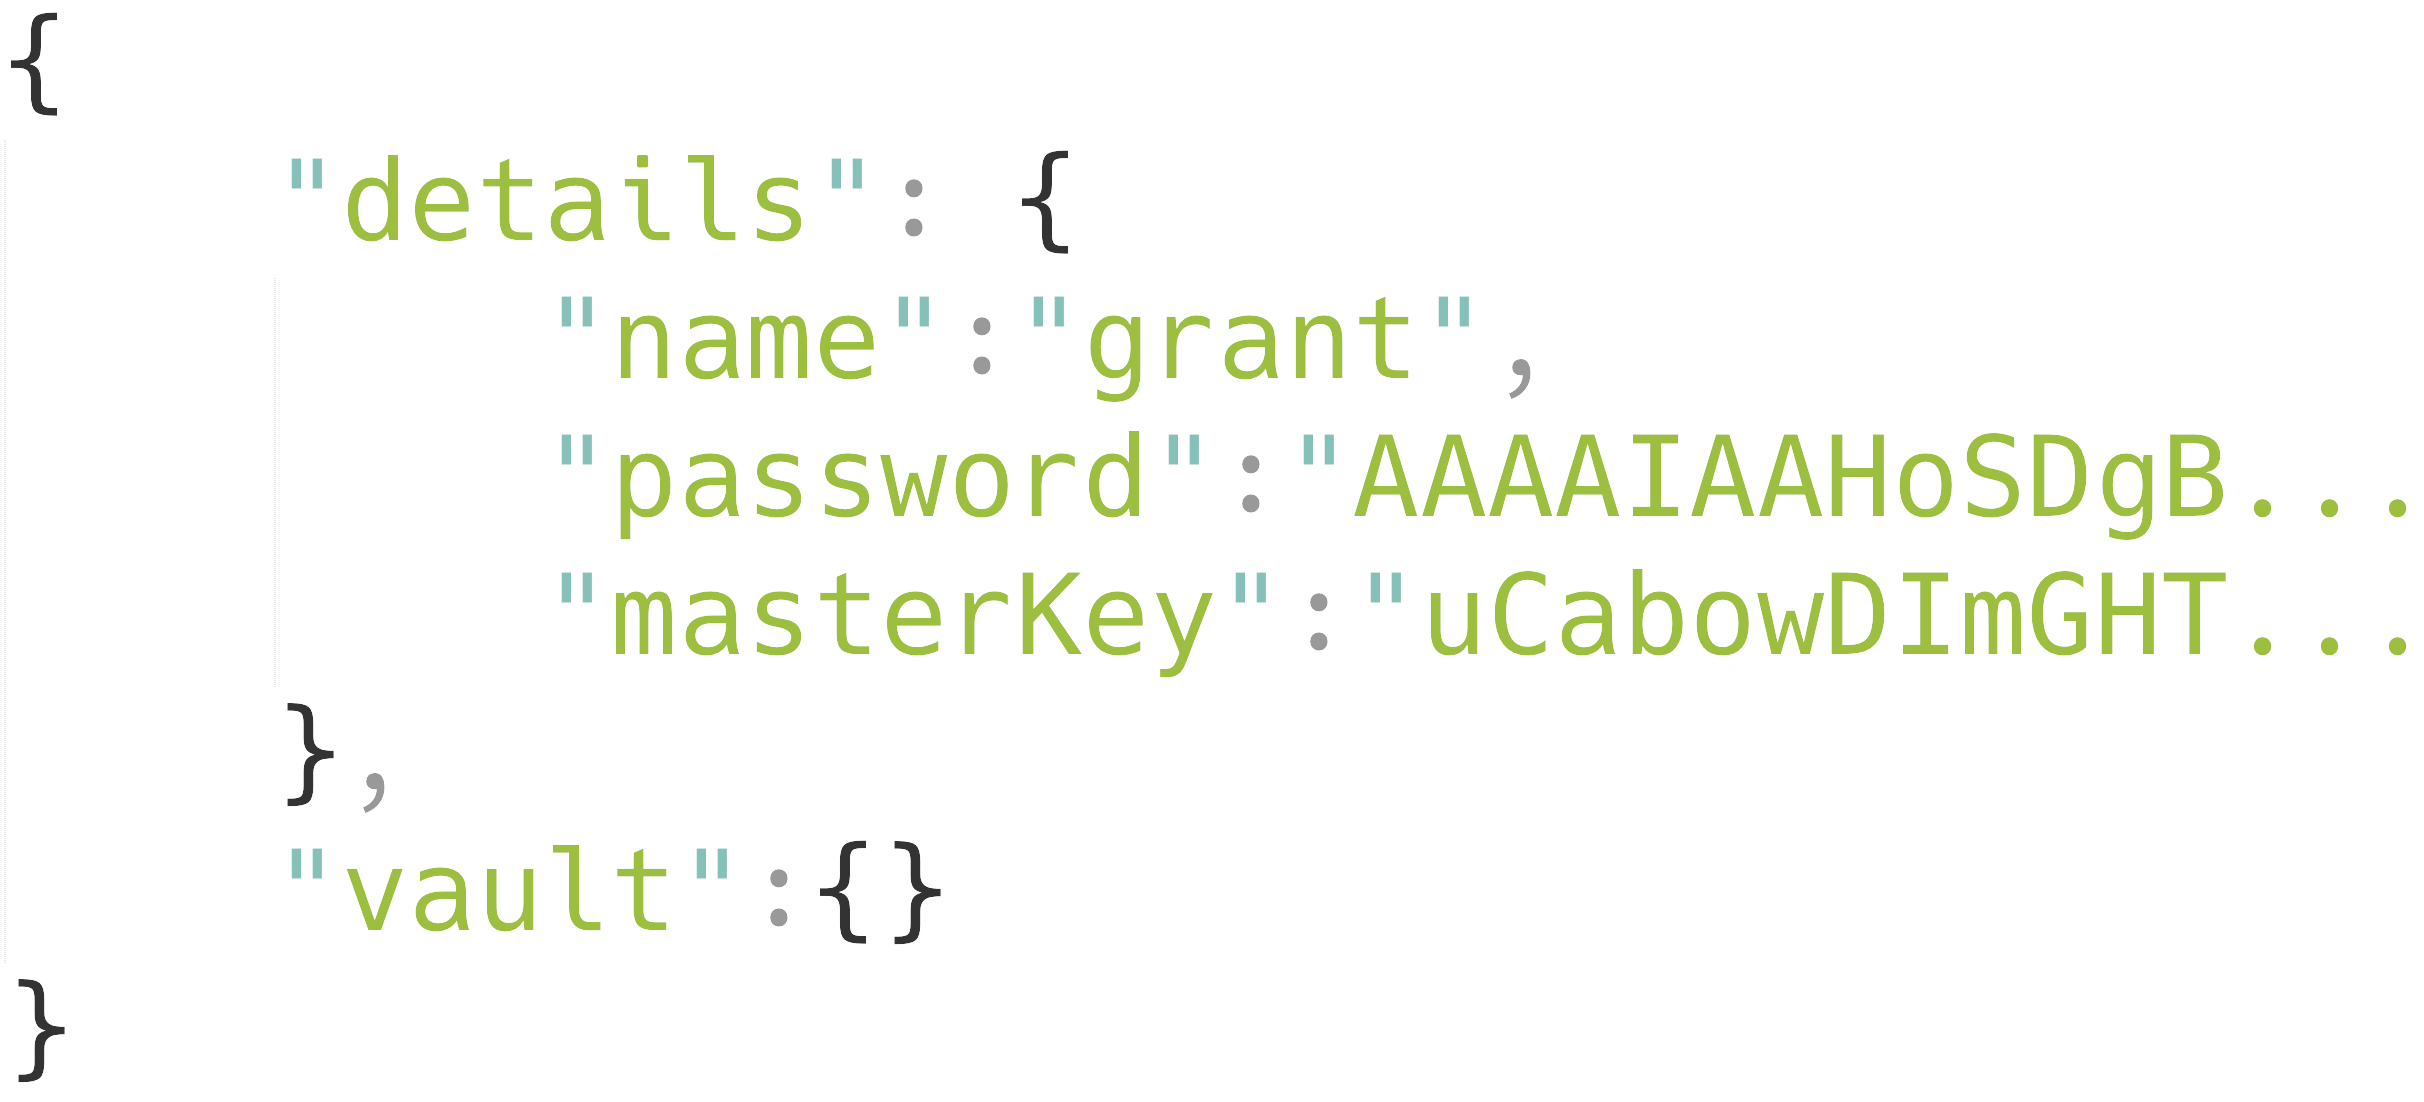
\includegraphics[scale=.35]{storage_format.png}

% BEGIN SYSTEM MODELING CHAPTER %
\chapter{System Modeling}

\section{Activity Diagrams}

\subsection{Login}
The login window is the first window that will a user will see as long as they have already created a profile previously. Login is a simple operation that involves taking the users username and password verifying that it matches the hashed version. Once authenticated the user will be forwarded to the main window. If a profile was not previously created on start Vaultron will ask you to create a profile, making sure the profile has not been taken before and the password is of sufficient length. Once that is done the user will be forwarded to the main window. This activity diagram models use case and 3.2.3 in the functional requirements section.

\vspace{4mm}
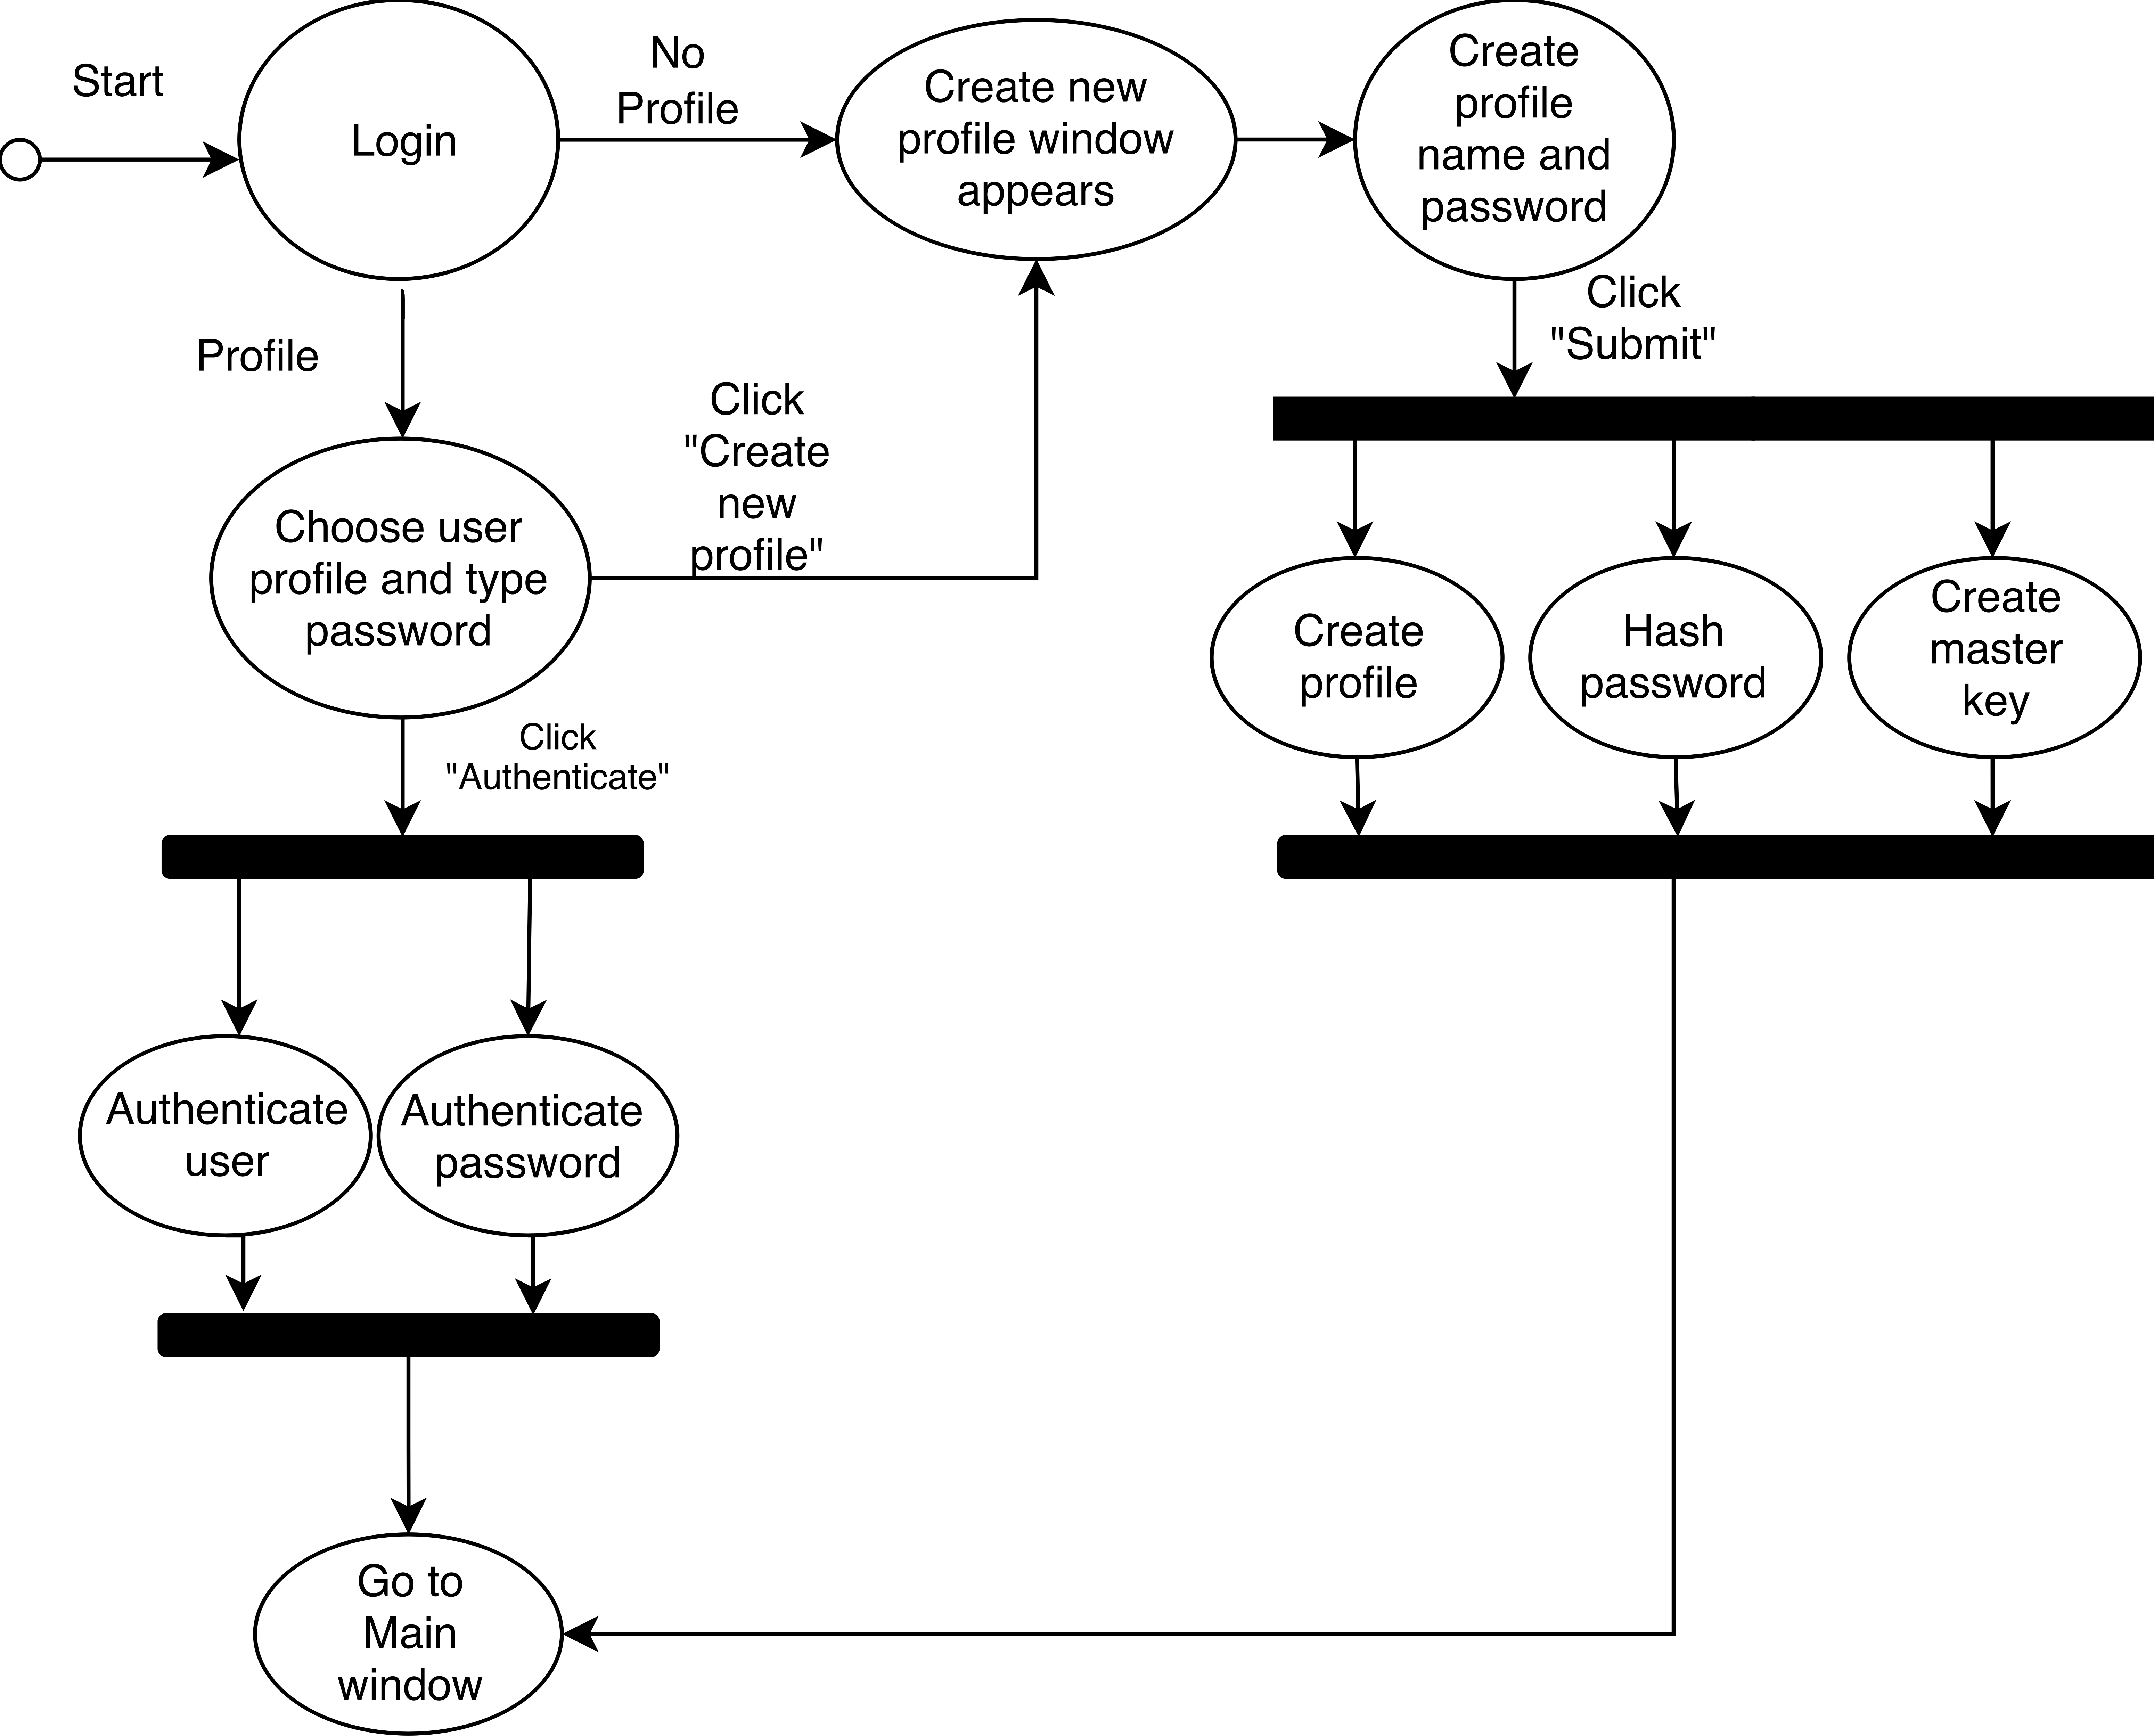
\includegraphics[scale=.076]{login_activity.png}

\clearpage

\subsection{Encrypt/Decrypt Entries}
Encryption and decryption of data are both accomplished using a master key that is encrypted using a hash of the users password. The master key in Vaultrons case is a 2048 bytes. This allows the encrypted data to have a large amount of entropy even if the users password is shorter. The master key is decrypted with the hash of the users password. This activity diagram models use case 3.2.2 in the functional requirements section.

\vspace{4mm}
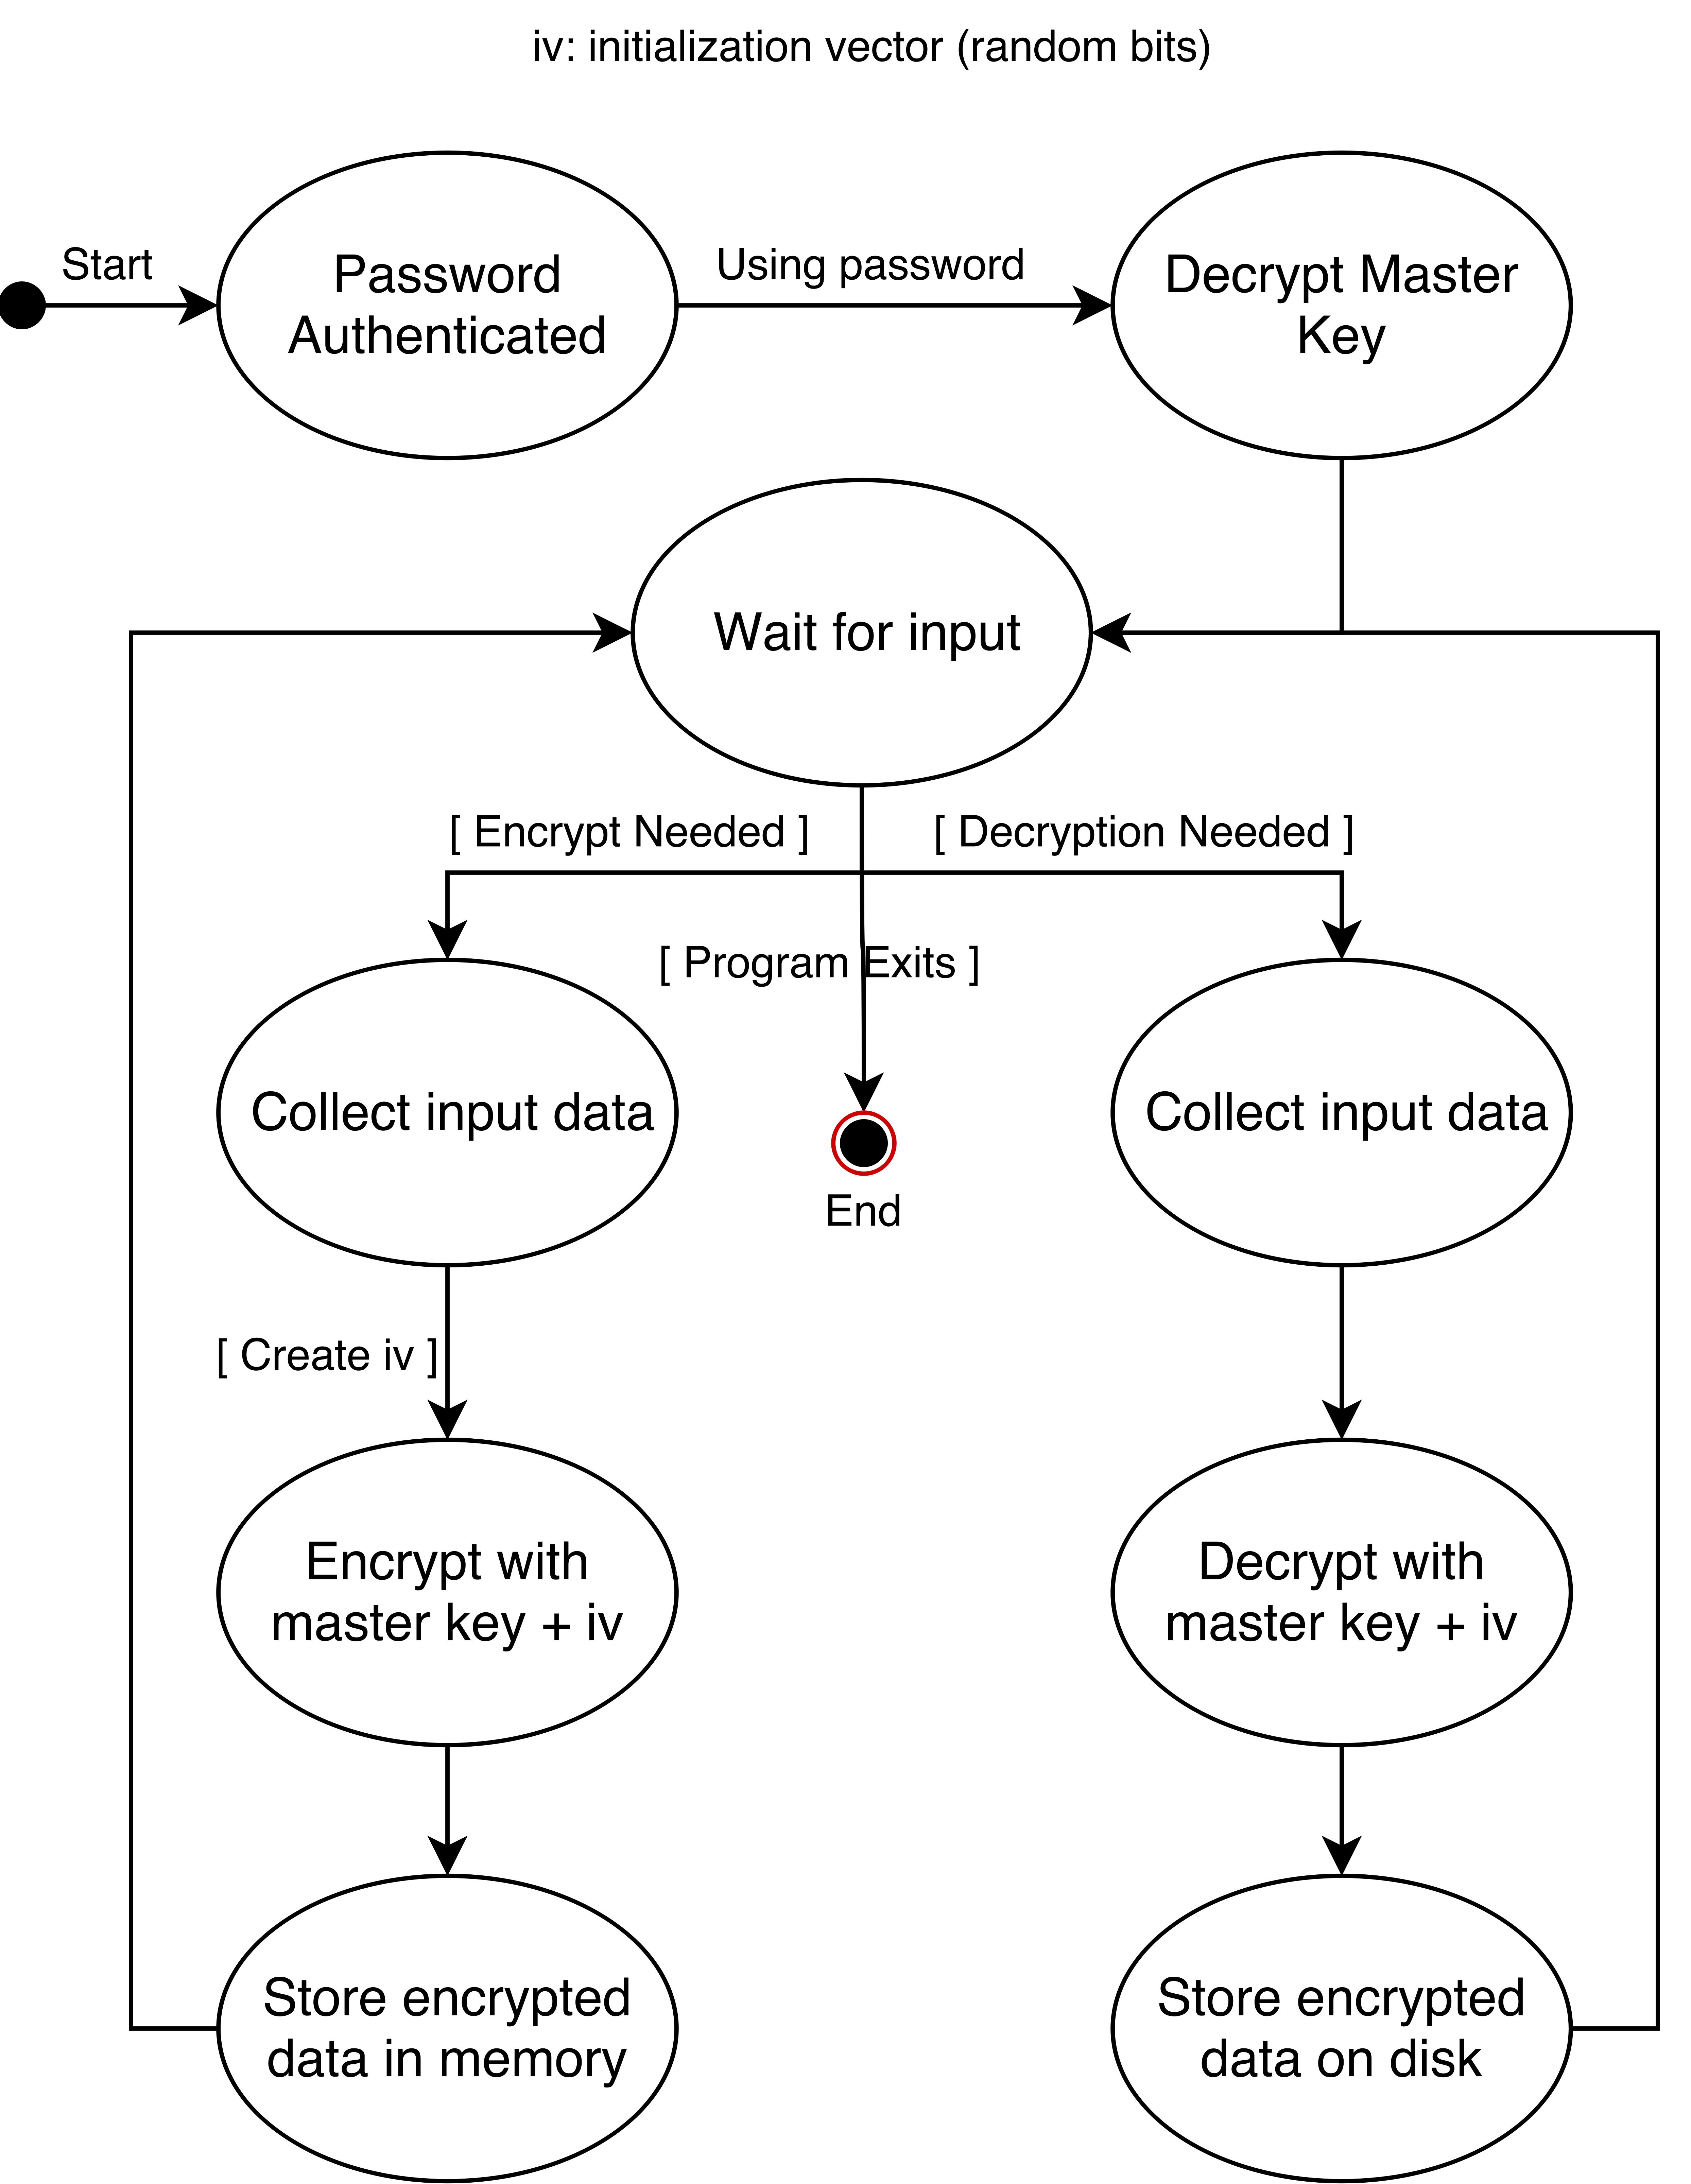
\includegraphics[scale=.075]{encryption.png}

\clearpage

\subsection{Add/Update Entry}
Adding an entry to the vault starts with clicking the Add Entry button. Then the user is asked for the entries information (website, username, password, etc). When the entry is submitted it is added to the users vault, if the entry is not new, the password is updated otherwise a new entry is created. This activity diagram models use case 3.2.5 in the functional requirements section.

\vspace{4mm}
\begin{center}
\includegraphics [scale=.5]{newEntry.png}
\end{center}

\clearpage

\subsection{Password Generator}
Password generation gives the user many options on what kind of password they want to create. When an option is changed the password is regenerated automatically with the new variables. All randomness used when generation the passwords is collected from a cryptographically secure source to ensure that there is no repetition with the kind of passwords that are generated. Once a suitable password has been chosen the copy button can be pressed to copy the password to the users clipboard. This activity diagram models use case 3.2.1 in the functional requirments section.

\vspace{4mm}
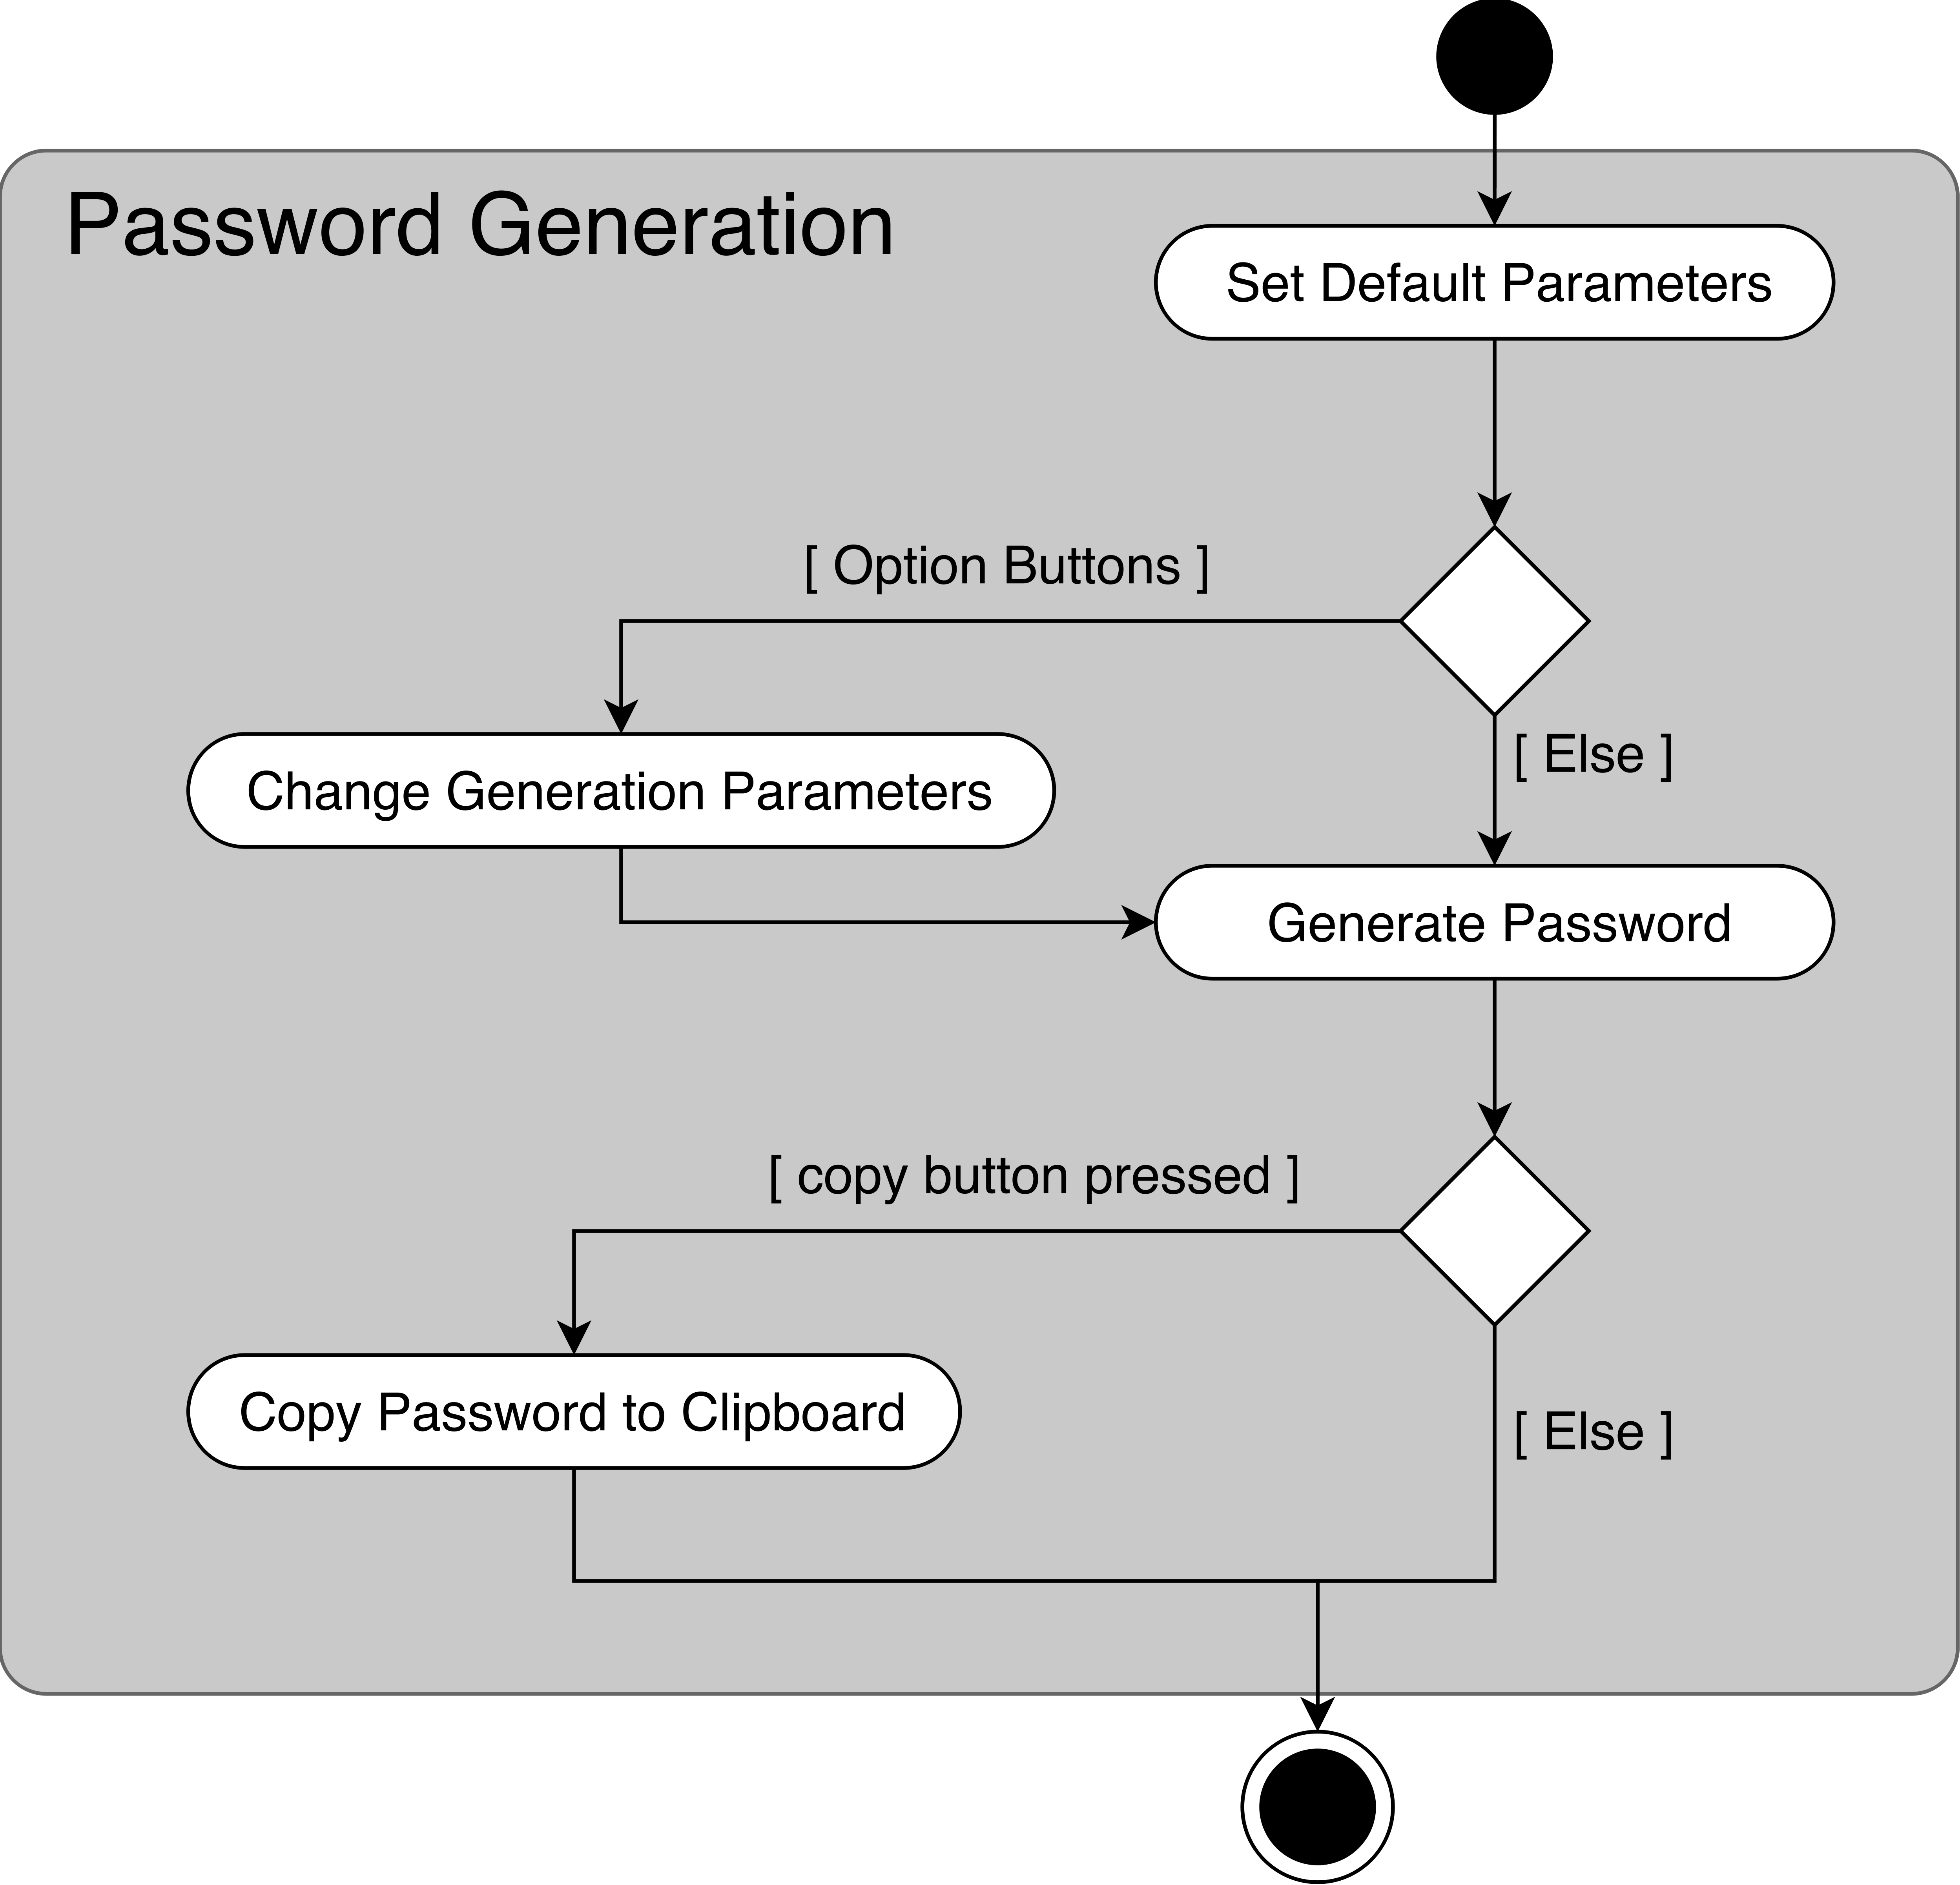
\includegraphics [scale=.09]{passgen.png}

\clearpage

\section{Structural Modeling}
Because our application is built using Electron, a JavaScript wrapper, 
the over setup of our app does not revolve around classes. Because of this
our class diagram displays the interaction of the CSS, HTML and JavaScript 
files with each other and briefly highlights the methods in each of the 
JavaScript files. In addition to this many of the functions in our code do
not return any values and instead either modify a element existing in one of
the HTML pages or send a message to the electron event listener. When an 
event with a particular title is received a function is called. These reasons
make JavaScript not a suitable language to develop class diagrams for, but
we present a generalized display of our program setup to accommodate a class
diagram.


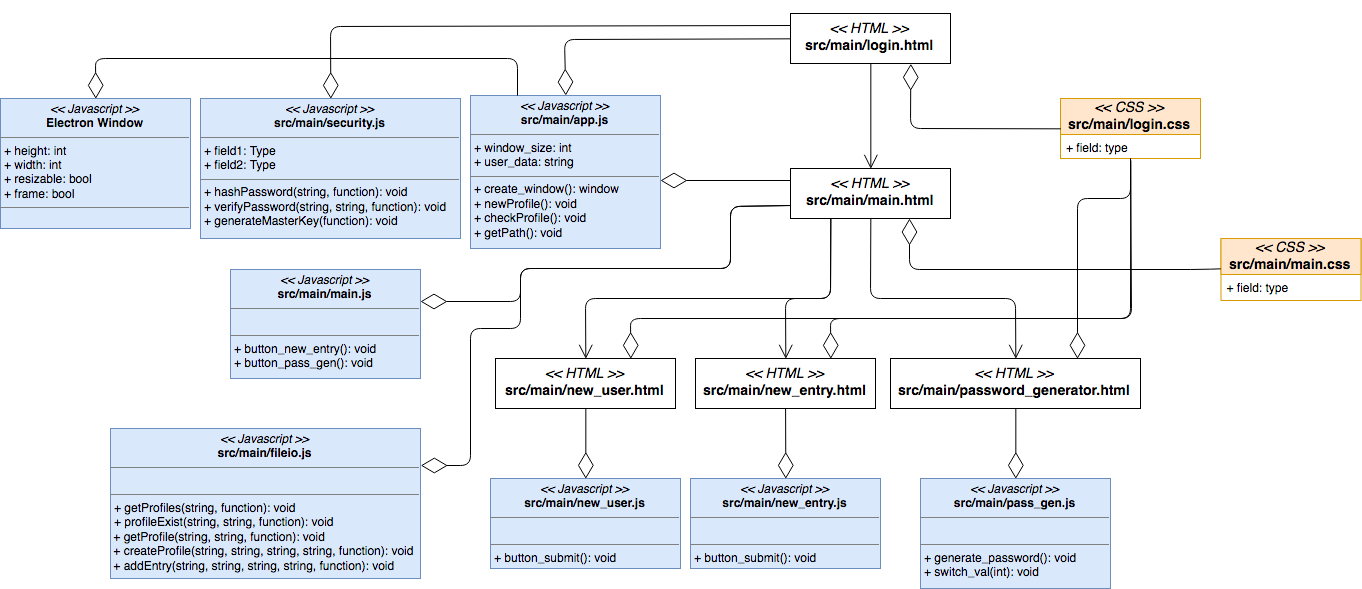
\includegraphics[scale=.1]{class_diagram.png}

\section{Behavior Modeling}
This state diagram overviews the high level layout of Vaultron. When started the user will be taken to the login screen. From their they can choose to create a new profile or to just login to a profile already available. Once logged in the user will be taken to the main window which displays a table of all of the entries within their vault. From the main window the user can either, generate a password, create a new entry, view and search their entries, and quit the application. Generating a password and creating a new entry both open a new window for the user to interact with. 


\includegraphics[scale=.1]{state_diagram.png}

\end{document}
